\documentclass{oblivoir}
%%%Default packages
\usepackage{amsmath,amssymb,amsthm,kotex,tabu,graphicx,pifont}
\usepackage{../kswrapfig}

\usepackage{gensymb} %\degree

%%%More packages
%\usepackage{caption,subcaption}
%\usepackage[perpage]{footmisc}
%
\usepackage[skipabove=10pt,innertopmargin=10pt,nobreak=true]{mdframed}

\usepackage[inline]{enumitem}
\setlist[enumerate,1]{label=(\arabic*)}
\setlist[enumerate,2]{label=(\alph*)}

\usepackage{multicol}
\setlength{\columnsep}{30pt}
\setlength{\columnseprule}{1pt}
%
%\usepackage{forest}
%\usetikzlibrary{shapes.geometric,arrows.meta,calc}
%
%%%defi theo exam prob rema proo
%이 환경들 아래에 문단을 쓸 경우 살짝 들여쓰기가 되므로 \hspace{-.7em}가 필요할 수 있다.

\newcounter{num}
\newcommand{\defi}[1]
{\noindent\refstepcounter{num}\textbf{정의 \arabic{num})} #1\par\noindent}
\newcommand{\theo}[1]
{\noindent\refstepcounter{num}\textbf{정리 \arabic{num})} #1\par\noindent}
\newcommand{\revi}[1]
{\noindent\refstepcounter{num}\textbf{복습 \arabic{num})} #1\par\noindent}
\newcommand{\exam}[1]
{\bigskip\bigskip\noindent\refstepcounter{num}\textbf{예시 \arabic{num})} #1\par\noindent}
\newcommand{\prob}[1]
{\bigskip\bigskip\noindent\refstepcounter{num}\textbf{문제 \arabic{num})} #1\par\noindent}
\newcommand{\rema}[1]
{\bigskip\bigskip\noindent\refstepcounter{num}\textbf{참고 \arabic{num})} #1\par\noindent}
\newcommand{\proo}
{\bigskip\noindent\textsf{증명)}}

\newenvironment{talign}
 {\let\displaystyle\textstyle\align}
 {\endalign}
\newenvironment{talign*}
 {\let\displaystyle\textstyle\csname align*\endcsname}
 {\endalign}
%
%%%Commands

\newcommand{\procedure}[1]{\begin{mdframed}\vspace{#1\textheight}\end{mdframed}}

\newcommand\an[1]{\par\bigskip\noindent\textbf{문제 \ref{#1})}\par\noindent}

\newcommand\ann[2]{\par\bigskip\noindent\textbf{문제 \ref{#1})}\:\:#2\par\medskip\noindent}

\newcommand\ans[1]{\begin{flushright}\textbf{답 : }#1\end{flushright}}

\newcommand\anssec[1]{\bigskip\bigskip\noindent{\large\bfseries#1}}

\newcommand{\pb}[1]%\Phantom + fBox
{\fbox{\phantom{\ensuremath{#1}}}}

\newcommand\ba{\,|\,}

\newcommand\ovv[1]{\ensuremath{\overline{#1}}}
\newcommand\ov[2]{\ensuremath{\overline{#1#2}}}
%
%%%% Settings
%\let\oldsection\section
%
%\renewcommand\section{\clearpage\oldsection}
%
%\let\emph\textsf
%
%\renewcommand{\arraystretch}{1.5}
%
%%%% Footnotes
%\makeatletter
%\def\@fnsymbol#1{\ensuremath{\ifcase#1\or
%*\or **\or ***\or
%\star\or\star\star\or\star\star\star\or
%\dagger\or\dagger\dagger\or\dagger\dagger\dagger
%\else\@ctrerr\fi}}
%
%\renewcommand{\thefootnote}{\fnsymbol{footnote}}
%\makeatother
%
%\makeatletter
%\AtBeginEnvironment{mdframed}{%
%\def\@fnsymbol#1{\ensuremath{\ifcase#1\or
%*\or **\or ***\or
%\star\or\star\star\or\star\star\star\or
%\dagger\or\dagger\dagger\or\dagger\dagger\dagger
%\else\@ctrerr\fi}}%
%}   
%\renewcommand\thempfootnote{\fnsymbol{mpfootnote}}
%\makeatother
%
%%% 객관식 선지
\newcommand\one{\ding{172}}
\newcommand\two{\ding{173}}
\newcommand\three{\ding{174}}
\newcommand\four{\ding{175}}
\newcommand\five{\ding{176}}
\usepackage{tabto,pifont}
%\TabPositions{0.2\textwidth,0.4\textwidth,0.6\textwidth,0.8\textwidth}

\newcommand\taba[5]{\par\noindent
\one\:{#1}
\tabto{0.2\textwidth}\two\:\:{#2}
\tabto{0.4\textwidth}\three\:\:{#3}
\tabto{0.6\textwidth}\four\:\:{#4}
\tabto{0.8\textwidth}\five\:\:{#5}}

\newcommand\tabb[5]{\par\noindent
\one\:{#1}
\tabto{0.33\textwidth}\two\:\:{#2}
\tabto{0.67\textwidth}\three\:\:{#3}\medskip\par\noindent
\four\:\:{#4}
\tabto{0.33\textwidth}\five\:\:{#5}}

\newcommand\tabc[5]{\par\noindent
\one\:{#1}
\tabto{0.5\textwidth}\two\:\:{#2}\medskip\par\noindent
\three\:\:{#3}
\tabto{0.5\textwidth}\four\:\:{#4}\medskip\par\noindent
\five\:\:{#5}}

\newcommand\tabd[5]{\par\noindent
\one\:{#1}\medskip\par\noindent
\two\:\:{#2}\medskip\par\noindent
\three\:\:{#3}\medskip\par\noindent
\four\:\:{#4}\medskip\par\noindent
\five\:\:{#5}}
%
%%%% fonts
%
%\usepackage{fontspec, xunicode, xltxtra}
%\setmainfont[]{은 바탕}
%\setsansfont[]{은 돋움}
%\setmonofont[]{은 바탕}
%\XeTeXlinebreaklocale "ko"
%%%%
\begin{document}

\title{수학 : 03 방정식과 부등식}
\author{}
\date{\today}
\maketitle
\tableofcontents
\newpage

%%%
\section{일차연립방정식}

%
\exam{}\label{system1}
\begin{align}
3x+2y-3&=0\\
x-y-1&=0
\end{align}

\((1)+2\times(2)\)를 하면,
\[5x-5=0\]
따라서 \(x=1\)이다.
이것을 \((1)\)에 대입하면
\[3\cdot1+2y-3=0\tag{3}\]
따라서 \(y=0\)이다.
\ans{\((x,y)=(1,0)\)}

이렇듯 주어진 식들에 일정한 숫자를 곱해 더하거나 빼서 답을 얻는 방법을 \emph{가감법}이라고 한다.
이 방법 말고도 \emph{대입법}이나 \emph{등치법}이 쓰일 수 있다.

\bigskip\bigskip\bigskip
\begin{minipage}{.45\textwidth}
\begin{mdframed}[frametitle=대입법]
(2)를 변형한
\[y=x-1\]
을 (1)에 대입하면
\[3x+2(x-1)-3=0\]
따라서 \(x=1\), \(y=0\).
\end{mdframed}
\end{minipage}
\begin{minipage}{.45\textwidth}
\begin{mdframed}[frametitle=등치법]
\vspace{-15pt}
\begin{align*}
y&=-\frac32x+\frac32\\
y&=x-1
\end{align*}
%\[-\frac32x+\frac32\stackrel{(1)}=y\stackrel{(2)}=x-1\]
로부터
\[-\frac32x+\frac32=x-1\]
따라서 \(x=1\), \(y=0\).
\end{mdframed}
\end{minipage}

\clearpage
%
\exam{}\label{system2}
\setcounter{equation}0
\begin{align}
2x+4y+1=0\\
x+2y+3=0
\end{align}

\((1)-2\times(2)\)를 하면,
\[0\cdot x+0\cdot y-5=0\tag{3}\]
이 된다.
\((3)\)을 만족시키는 \(x\), \(y\)는 존재하지 않는다.
따라서 이 연립방정식의 해는 없다.
\ans{근이 없다(불능不能)}

%
\exam{}\label{system3}
\setcounter{equation}0
\begin{align}
2x+4y+6=0\\
x+2y+3=0
\end{align}

\((1)-2\times(2)\)를 하면,
\begin{equation}
0\cdot x+0\cdot y+0=0
\end{equation}
이 된다.
\((3)\)은 항상 성립하는 식이다.
\(x\)가 하나 주어졌을 때 \(y\)값은 \(y=-\frac12x-\frac32\)로 주어진다.
예를 들어 \(x=0\)이면 \(y=-\frac32\), \(x=1\)이면 \(y=-2\), \(x=2\)이면 \(y=-\frac52\)이다.
즉,
\[(x,y)=\left(0,-\frac32\right),\left(1,-2\right),\left(2,-\frac52\right),\cdots\]
등이 해가 될 수 있다.
따라서 이 연립방정식의 해는 무수히 많다.
\ans{근이 무수히 많다(부정不定)}%\\ \((x,y)=\left(x,-\frac12x-\frac32\right)\)}

\clearpage

%
\rema{}
예시 \ref{system1})--\ref{system3})를 그래프로 해석해보자.
예시 \ref{system1})의 (1)과 (2)를 변형하면
\begin{align*}
y=-\frac32x+\frac32\\
y=x-1
\end{align*}
이 되어
(1)은 기울기가 \(-\frac32\)이고 \(y\)절편이 \(\frac32\)인 직선,
(2)는 기울기가 \(1\)이고 \(y\)절편이 \(-1\)인 직선이 된다.
두 직선은 한 점 \((1,0)\)에서 만나므로 연립방정식을 만족하는 \((x,y)\)는 한 개이다.

\begin{center}
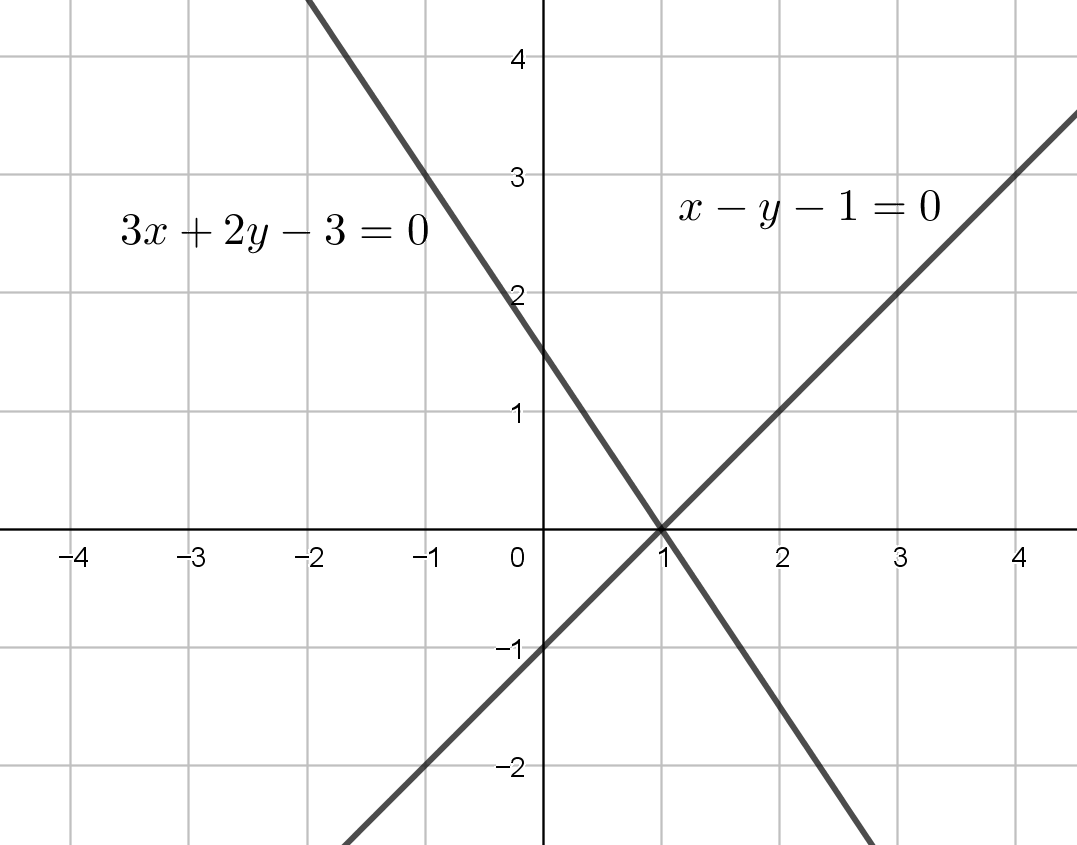
\includegraphics{system_examples_01}
\end{center}

\clearpage
한편, 예시 \ref{system2})의 경우 두 직선이 평행하므로 서로 만나지 않는다.
즉, 두 직선의 교점이 없다.
따라서 연립방정식을 만족시키는 \((x,y)\)는 존재하지 않는다.

\begin{center}
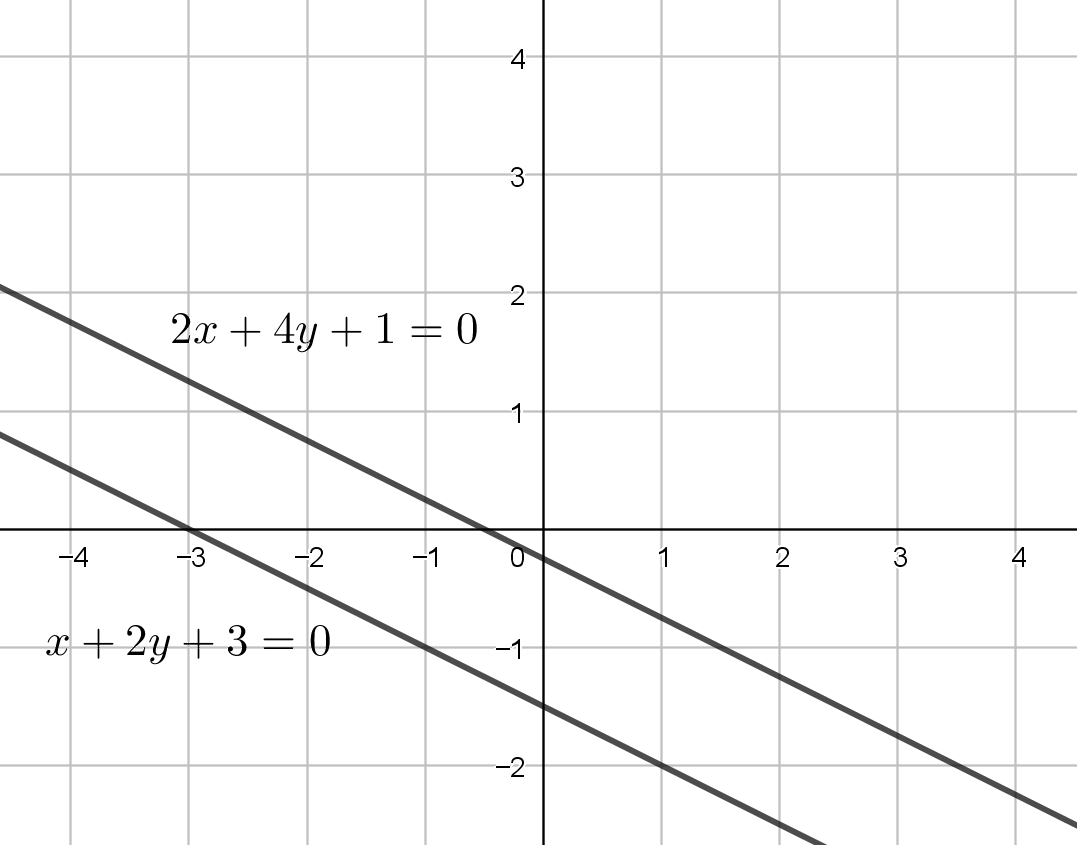
\includegraphics{system_examples_02}
\end{center}

또한, 예시 \ref{system3})에서는 두 직선이 일치한다.
즉 두 직선의 교점이 무한히 많다.
따라서 연립방정식을 만족시키는 \((x,y)\)는 무한히 많다.

\begin{center}
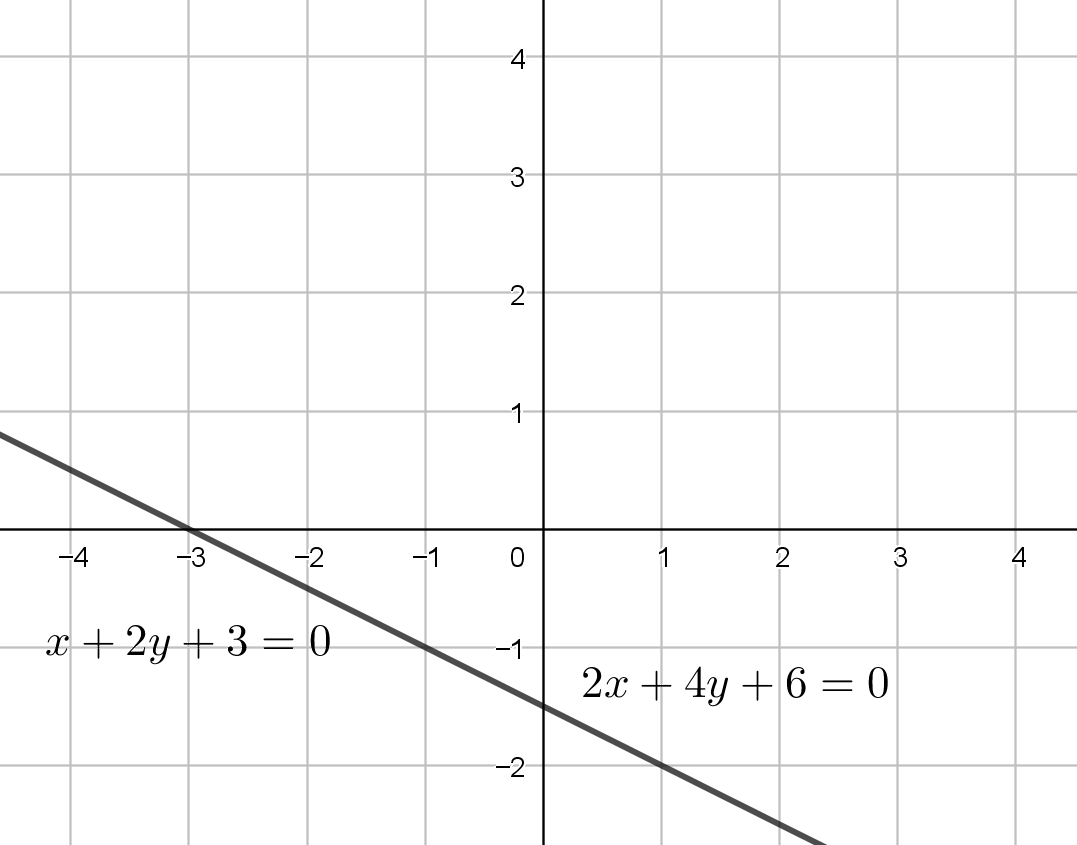
\includegraphics{system_examples_03}
\end{center}

\begin{mdframed}
%
\theo{}\label{theo_system}
\(a\), \(b\), \(c\), \(a'\), \(b'\), \(c'\)가 \(0\)이 아닌 실수일 때,
연립방정식
\[
\begin{cases}
ax+by+c=0\\
a'x+b'y+c'=0
\end{cases}
\]
의 근은 다음과 같다.
\begin{enumerate}[label=\emph{\roman*})]
\item
\(\frac a{a'}\neq\frac b{b'}\)이면 근이 한 개이다.
\item
\(\frac a{a'}=\frac b{b'}\neq\frac c{c'}\)이면 근이 없다.
\item
\(\frac a{a'}=\frac b{b'}=\frac c{c'}\)이면 근이 무수히 많다.
\end{enumerate}
\end{mdframed}

%
\proo
두 식을 각각 정리하면
\[
\begin{cases}
y=-\frac bax-\frac ca\\
y=-\frac{b'}{a'}x-\frac{c'}{a'}
\end{cases}
\]
이다.
\(\frac a{a'}=\frac b{b'}\)를 변형하면
\[-\frac ba=-\frac{b'}{a'}\]
이 된다.
또한
\(\frac a{a'}=\frac c{c'}\)를 변형하면
\[-\frac ca=-\frac{c'}{a'}\]
이 된다.
즉 \(\frac a{a'}=\frac b{b'}\)아면 두 직선의 기울기가 같고, \(\frac a{a'}=\frac c{c'}\)이면 두 직선의 \(y\)절편이 같다.

\bigskip
i)의 경우, 두 직선의 기울기가 서로 다르다.
따라서 두 직선은 한 점에서 만나고 연립방정식의 근은 한 개이다.

\bigskip
ii)의 경우, 두 직선의 기울기가 서로 같고 \(y\)절편은 서로 다르다.
따라서 두 직선은 평행하여 만나지 않는다.
그러므로 연립방정식의 근은 없다.

\bigskip
iii)의 경우, 두 직선의 기울기가 서로 같고 \(y\)절편도 서로 같다.
따라서 두 직선은 일치하여 무수히 많은 점에서 만난다.
그러므로 연립방정식의 근은 무수히 많다.

%
\prob{}\label{proof2}
다음은 가감법을 이용하여 정리 \ref{theo_system})를 증명한 것이다.
(가), (나), (다)에 알맞은 것을 채워넣어라.

\proo
\setcounter{equation}{0}
\begin{gather}
ax+by+c=0\\
a'x+b'y+c'=0
\end{gather}
(1)에는 \(b'\)을 곱하고, (2)에는 \(b\)를 곱하면
\begin{gather}
ab'x+bb'y+b'c=0\\
\fbox{\phantom{a'bx+}(가)\phantom{+bc'}}=0
%\pb{a'bx+bb'y+bc'}=0
\end{gather}
이 된다.
\((3)-(4)\)를 하면
\begin{equation}
(ab'-a'b)x+(b'c-bc')=0
\end{equation}
이 된다.

\bigskip
i)의 경우,
\(\frac a{a'}\neq\frac b{b'}\)로부터 \(ab'-a'b\neq0\)이다.
따라서 (5)를 \(ab'-a'b\)로 나누어 정리하면
\begin{equation}
x=\fbox{\phantom{\(\frac aa\)}(나)\phantom{\(\frac aa\)}}
%\pb{\frac{bc'-b'c}{ab'-a'b}}
\end{equation}
이다.
이제 (6)을 (1)에 대입하면
\[a\cdot\fbox{\phantom{\(\frac aa\)}(나)\phantom{\(\frac aa\)}}+by+c=0\]
이고, 이것을 정리하면
\begin{align*}
by
&=-a\cdot\fbox{\phantom{\(\frac aa\)}(나)\phantom{\(\frac aa\)}}-c\\
&=\frac{-a(bc'-b'c)-(ab'-a'b)c}{ab'-a'b}\\
&=\frac{a'bc-abc'}{ab'-a'b}
\end{align*}
따라서
\[y=\fbox{\phantom{\(\frac aa\)}(다)\phantom{\(\frac aa\)}}\]
이다.
즉 연립방정식의 근은
\[
(x,y)=\left(\:\fbox{\phantom{\(\frac aa\)}(나)\phantom{\(\frac aa\)}}\:\:,\:\:\fbox{\phantom{\(\frac aa\)}(다)\phantom{\(\frac aa\)}}\:\right)
\]
의 한 개이다.

\bigskip
ii)와 iii)의 경우,
\(\frac a{a'}=\frac b{b'}\)로부터 \(ab'-a'b=0\)이다.
따라서 (5)는
\begin{equation}
0\cdot x+(b'c-bc')=0
\end{equation}
이다.

\bigskip
ii)이면 \(b'c-bc'\neq0\)이므로 (7)의 근은 없다.
따라서 연립방정식의 근도 없다.
또, iii)이면 \(b'c-bc'=0\)이므로 (7)은 무수히 많은 근을 가진다.
따라서 연립방정식도 무수히 많은 근을 가진다.

\clearpage

%
\prob{다음 연립방정식을 풀어라.}\label{system_problem1}
\begin{enumerate}
\item
\(\begin{cases}
x+2y=5\\
2x+y=4
\end{cases}\)
\item
\(\begin{cases}
x-2y=3\\
2x+4y=14
\end{cases}\)
\item
\(\begin{cases}
2x-3y=5\\
-4x+6y=-10
\end{cases}\)
\item
\(\begin{cases}
x+3y=4\\
3x+9y=12
\end{cases}\)
\end{enumerate}

%
\prob{다음 연립방정식이 해를 가지지 않을 때, \(k\)의 값을 구하여라.}\label{system_problem2}
\(\begin{cases}
2x+y+5=0\\
x+ky+1=0
\end{cases}\)

%
\prob{다음 연립방정식이 무수히 많은 해를 가질 때, \(k\)의 값을 구하여라.}\label{system_problem3}
\(\begin{cases}
x-y+3=0\\
-2x+2y+k=0
\end{cases}\)

%%%
\section{이차부등식}

%
\exam{}\label{D>0}
다음 이차부등식들의 해를 구하여라.
\begin{enumerate}
\item
\(x^2-2x-3>0\)
\item
\(x^2-2x-3<0\)
\end{enumerate}

\begin{mdframed}[frametitle=풀이1]
\vspace{-20pt}
\begin{align*}
AB>0\iff&(A>0\:이고\:\:B>0)\:\:또는\:\:(A<0\:이고\:\:B<0)\\
AB<0\iff&(A>0\:이고\:\:B<0)\:\:또는\:\:(A<0\:이고\:\:B>0)
\end{align*}
임을 이용한다.

\bigskip\bigskip
(1) \((x-3)(x+1)>0\)에서
\begin{align*}
&(x-3>0\:이고\:\:x+1>0)\:\:또는\:\:(x-3<0\:이고\:\:x+1<0)\\
\iff
&(x>3\:이고\:\:x>-1)\:\:또는\:\:(x<3\:이고\:\:x>-1)\\
\iff
&x>3\:\:또는\:\:x>-1
\end{align*}
이다.

\bigskip\bigskip
(2) \((x-3)(x+1)<0\)에서
\begin{align*}
&(x-3\:이고\:\:x+1>0)\:\:또는\:\:(x-3>0\:이고\:\:x+1<0)\\
\iff
&(x<3\:이고\:\:x>-1)\:\:또는\:\:(x>3\:이고\:\:x<-1)\\
\iff
&-1<x<3\:\:또는\:\:(모순)\\
\iff
&-1<x<3
\end{align*}
이다.
\end{mdframed}


\begin{mdframed}[frametitle=풀이2]
\(y=x^2-2x-3\)의 그래프를 그리면 아래와 같다.
\begin{center}
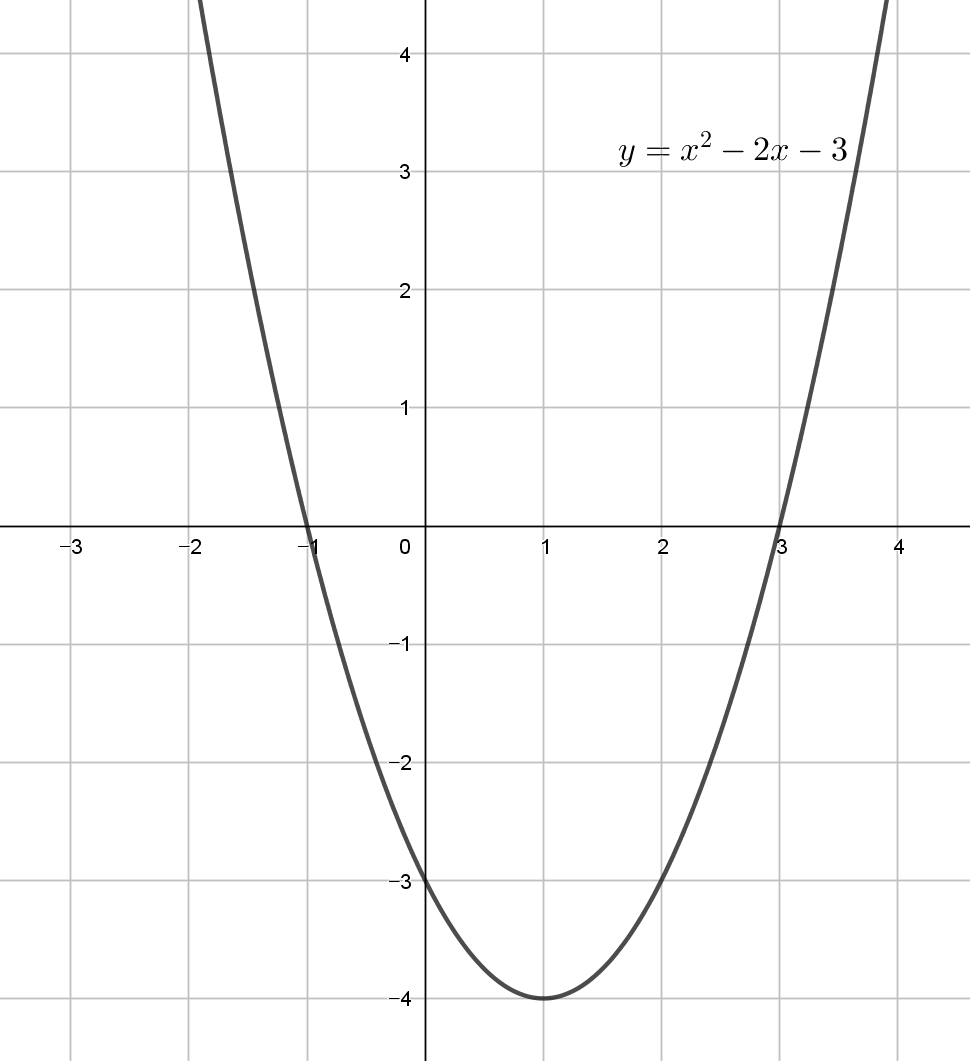
\includegraphics[width=0.5\textwidth]{y=x^2-2x-3}
\end{center}

(1)
그래프가 \(x\)축보다 위쪽에 있으려면 \(x<-1\) 또는 \(x>3\)이어야 한다.

(2)
그래프가 \(x\)축보다 아래쪽에 있으려면 \(-1<x<3\)이어야 한다.
\end{mdframed}
{\par\raggedleft\textbf{답 : }
(1) \(x<-1\) 또는 \(x>3\),\quad (2) \(-1<x<3\)
\par}

\clearpage
%
\prob{}\label{ineq1}
다음 이차부등식을 풀어라.
\begin{enumerate}
\item
\(x^2-x-12\ge0\)
\item
\(x^2-x-12\le0\)
\end{enumerate}
\begin{mdframed}[frametitle=풀이1]
\vspace{0.3\textheight}
\end{mdframed}
\begin{mdframed}[frametitle=풀이2]
\vspace{0.3\textheight}
\end{mdframed}

\clearpage
%
\exam{}\label{D<0}
다음 이차부등식들의 해를 구하여라.
\begin{enumerate}
\item
\(x^2+4x+4>0\)
\item
\(x^2+4x+4<0\)
\item
\(x^2-3x+3>0\)
\item
\(x^2-3x+3<0\)
\end{enumerate}

\begin{mdframed}[frametitle=풀이1]
\begin{center}
A가 실수일 때, \(A\ge0\)
\end{center}
임을 이용한다.

\begin{enumerate}
\item
주어진 식을 정리하면 \[(x+2)^2>0\]이고, 이 식은 \(x\neq-2\)이면 성립한다.
따라서 이 이차부등식의 해는 \(x\neq-2\)이다.
\item
주어진 식을 정리하면 \[(x+2)^2<0\]이고, 이 식은 성립하지 않는다.
따라서 이 이차부등식의 해는 없다.
\item
주어진 식을 정리하면 \[\left(x-\frac32\right)^2+\frac34>0\]이고, 이 식은 항상 성립한다.
따라서 이 이차부등식의 해는 모든 실수이다.
\item
주어진 식을 정리하면 \[\left(x-\frac32\right)^2+\frac34<0\]이고, 이 식은 성립하지 않는다.
따라서 이 이차부등식의 해는 없다.
\end{enumerate}
\end{mdframed}


\begin{mdframed}[frametitle=풀이2]
\(y=x^2+4x+4\)의 그래프를 그리면 아래와 같다.
\begin{center}
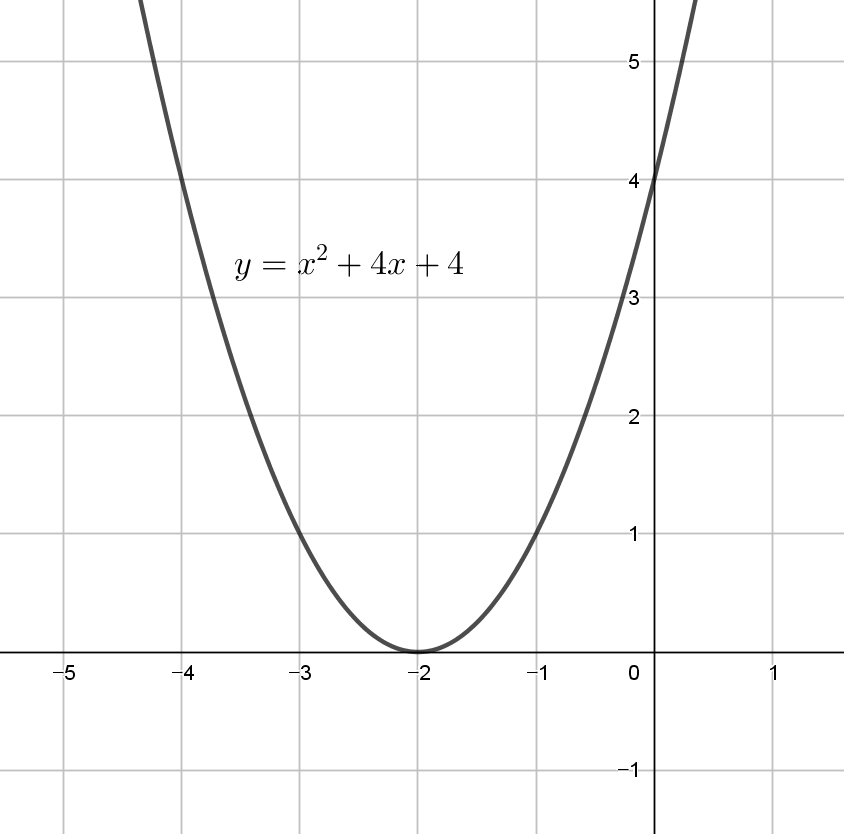
\includegraphics[width=0.45\textwidth]{y=x^2-4x+4}
\end{center}

(1)
그래프가 \(x\)축보다 위쪽에 있으려면 \(x\neq-2\)이면 된다.

(2)
그래프가 \(x\)축보다 아래쪽에 있는 경우는 없다.

\bigskip\noindent
\(y=x^2+3x+3\)의 그래프를 그리면 아래와 같다.
\begin{center}
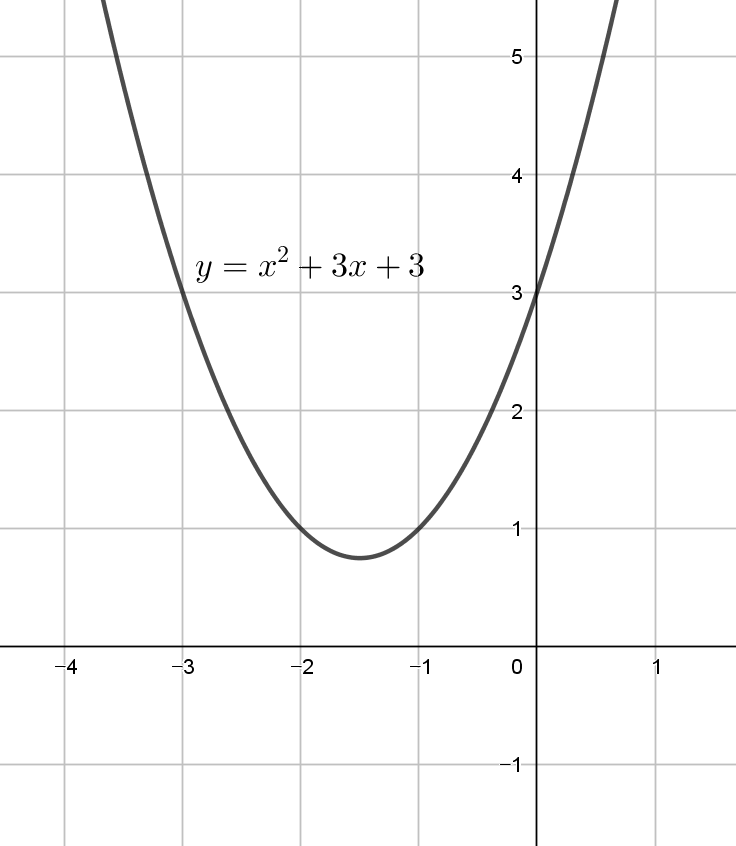
\includegraphics[width=0.45\textwidth]{y=x^2+3x+3}
\end{center}

(3)
그래프는 \(x\)축보다 항상 위쪽에 있다.

(4)
그래프가 \(x\)축보다 아래쪽에 있는 경우는 없다.
\end{mdframed}
{\par\raggedleft\textbf{답 : }
(1) \(x\)는 \(x\neq-2\)인 모든 실수,\quad (2) 해는 없다\\
(3) \(x\)는 모든 실수,\quad (4) 해는 없다
\par}

\clearpage
%
\prob{}\label{ineq2}
다음 이차부등식을 풀어라.
\begin{enumerate}
\item
\(x^2-2x+1>0\)
\item
\(x^2-2x+1\ge0\)
\item
\(x^2-2x+1<0\)
\item
\(x^2-2x+1\le0\)
\end{enumerate}
\begin{mdframed}[frametitle=풀이1]
\vspace{0.3\textheight}
\end{mdframed}
\begin{mdframed}[frametitle=풀이2]
\vspace{0.3\textheight}
\end{mdframed}

%
\exam{}
모든 실수 \(x\)에 대하여
\[x^2-3x+k>0\]
이 성립하도록 하는 \(k\)의 범위를 구하여라.
\begin{mdframed}[frametitle=풀이]
\(f(x)\)를
\[f(x)=x^2-3x+k\]
로 두면 \(y=f(x)\)의 그래프는 아래로 볼록인 포물선이다.
모든 실수 \(x\)에 대해 \(f(x)>0\)이려면 \(y=f(x)\)의 그래프가 \(x\)축보다 위에 있어야 한다.
즉 \(y=f(x)\)의 그래프와 \(x\)축이 서로 만나지 않아야 하므로 방정식 \(f(x)=0\)의 실근이 없어야 한다.
그러므로 \(D<0\)를 풀면,
\[D=9-4k<0\]
따라서
\(k>\frac94\)이다.
\end{mdframed}

%
\prob{}\label{ineq3}
모든 실수 \(x\)에 대하여
\[x^2+4x+k\ge0\]
이 성립하도록 하는 \(k\)의 범위를 구하여라.

%
\prob{}\label{ineq4}
모든 실수 \(x\)에 대하여
\[x^2+kx+3>0\]
이 성립하도록 하는 \(k\)의 범위를 구하여라.



%%
\section*{답}
\addcontentsline{toc}{chapter}{\protect\numberline{*}답}

\begin{minipage}[t]{.49\textwidth}
%
\an{system_problem1}
\begin{enumerate}
\item
\((x,y)=(1,2)\)
\item
\((x,y)=(5,1)\)
\item
근이 무수히 많다(부정)\\
\((x,y)=\left(x,\frac23x-\frac53\right)\)
\item
근이 없다(불능)
\end{enumerate}

%
\an{system_problem2}
\(4\)

%
\an{system_problem3}
\(-6\)

%
\an{proof2}
\begin{enumerate}
\item[(가)]
\(a'bx+bb'y+bc'\)
\item[(나)]
\(\frac{bc'-b'c}{ab'-a'b}\)
\item[(다)]
\(\frac{a'c-ac'}{ab'-a'b}\)
\end{enumerate}
%\((가)=a'bx+bb'y+bc'\)\\
%\((나)=\frac{bc'-b'c}{ab'-a'b}\)\\
%\((다)=\frac{a'c-ac'}{ab'-a'b}\)
\end{minipage}
%%
\begin{minipage}[t]{0.49\textwidth}
%
\an{ineq1}
\begin{enumerate}
\item
\(x\le-3\) 또는 \(x\ge4\)
\item
\(-3\le x\le 4\)
\end{enumerate}

%
\an{ineq2}
\begin{enumerate}
\item
\(x\)는 \(x\neq1\)인 모든 실수
\item
\(x\)는 모든 실수
\item
해는 없다.
\item
\(x=1\)
\end{enumerate}

%
\an{ineq3}
\(k\ge4\)

%
\an{ineq4}
\(-2\sqrt3<k<2\sqrt3\)
\end{minipage}

\end{document}